\documentclass{tmr}

\usepackage{amsmath}
\usepackage[utf8]{inputenc}

\title{Enumeration of Tuples with Hyperplanes} % Avoid extreme use of enumerations (to quote the guidelines of the Monad Reader)
\author{Tillmann Vogt\email{tillk.vogt@googlemail.com}}

\newcommand{\authornote}[3]{{\color{#2} {\sc #1}: #3}}
\newcommand\bay[1]{\authornote{edward}{blue}{#1}}
\newcommand\tkv[1]{\authornote{Tillmann}{green}{#1}}

\begin{document}

\begin{introduction}
%\bay{I rewrote the introduction. You're welcome to replace my introduction with an alternative; keep an eye out for flow.} \tkv{Some of your corrections make sense, I hope you kike the rewrite)}
Enumeration means assigning an integer value to a structure or, looking at the Haskell Prelude, defining an Enum instance. There are Enum instances for basic types like Bool or Char. But why are there no Enum instances for tuples?  Given that the elements of a tuple are enumerable, the combination ought to be enumerable too. Unfortunately it takes  too long to \eg enumerate all 7-tuples of Chars to find ''Haskell''. Another problem is that the classic method (imagine a counter ticking upwards) lets the digits increase with different speed and is therefore unusable for combinatorial problems where you want a quick variation of every digit. The solution that people most of the time chose in such a situation is a random function. The problem with a random function (apart from not being side effect free) is that you never have the confidence of having examined at least a defined part of the search space exhaustively. Using an enumeration like we present here, you can halt the processing \eg in a proofing system or for genetic algorithms, see how long it took to compute, maybe add constraints, and continue with the assurance of not having missed something. In this article we will describe a method how to enumerate tuples in a fair manner that could be used in such cases.
\end{introduction}

\subsection{Cartesian product of small sets}

The most straight forward way to enumerate tuples is to generate all combinations of elements of (finite) sets like this:
\begin{Verbatim}
cartProd (set:sets) = let cp = cartProd sets
                      in [x:xs | x <- set, xs <- cp]
cartProd [] = [[]]
\end{Verbatim}
This is a Cartesian product in maths, which can be found in the library haskell-for-maths. The exact way how the sets are enumerated does not matter because usually every element is used.

To understand what this function does, let's look at an example:

\begin{Verbatim}
cartProd [[0..3],[0..3],[0..3]],
\end{Verbatim}
evaluates to:
\begin{Verbatim}
[[0,0,0],
 [0,0,1],
 [0,0,2],
 [0,0,3],
 [0,1,0],
 [0,1,1],
 [0,1,2], ...].
\end{Verbatim}

One can see that this is counting of numbers with base 4.
This is fine if every combination has to be examined and the sets are small. If the sets become too big there is no way to go through all combinations. %\bay{Are we only looking at the first few elements of the permutation?}
In that case, this enumeration is problematic for several reasons:
\begin{enumerate}
\item It is not able to enumerate an infinite set at one of its digits. For example \begin{verbatim} cartProd [[0..3],[0..3],repeat 0] \end{verbatim} will only produce lists of [0,0,0] because it is stuck in the third list that contains infinitely many 0s. %\bay{This is unclear: what does it mean to "enumerate an infinite set"? (What you mean is that for every element which is a member of the enumeration, it will occur in the enumeration in finite time, or something similar.)  Also, this is a degenerate case of point 2.}
\item It does not distribute the changes fairly among the digits. The above enumeration is a lexicographic ordering that changes the last digit in the tuple all the time and the first rarely. In the next subsection we will see an enumeration (repeated diagonalization) that solves the first point but not this point.
\item Every set has to be of the same type, because it is a list. This limitation could be easily changed by transforming the lists into tuples and maybe do a lookup with the integer values in a table . %\bay{Maybe mention tuples here?}
\end{enumerate}

\subsection{Enumerating $\mathbb{Q} $}
There is another way to enumerate tuples that every computer scientist learns when showing that the rational numbers are enumerable. A rational number can be enumerated by giving an axis of natural numbers to each numerator and denominator. Then an enumeration is a path consisting of increasingly longer diagonals (Figure \ref{enum2}). For a way to avoid duplicates in this enumeration (like $2/2$) see \cite{rationals}.

\begin{figure}[htbp]
  \centering
     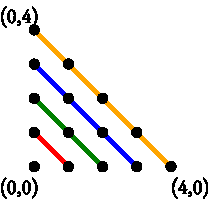
\includegraphics[width=0.25\textwidth]{enum2c.pdf}
  \caption{Enumeration of 2-tuples}
  \label{enum2}
\end{figure}

%\bay{I like these two sentences. :-)}
The next question, typically raised in an exercise course, is how to enumerate 3-tuples.
While everybody is thinking hard about a path through three dimensional space, somebody suggests to use the 2-tuples as a new axis and do the same diagonalization again. This is better than the former solution, %\bay{Might be clearer to explicitly say what the formal solution is.}
because it allows infinite sets in the digits (here $\mathbb{N}$), but there are many more 2-tuples  than single values ($O(x^2)$ against $O(x)$, $x$ being the size of each set at a digit), which again results in an unfair distribution (see the left picture of Figure \ref{enum3} that shows the path that is biased towards one axis). Doing this repeatedly results in distributions where one digit grows with $O(x^3)$ for 4-tuples, $O(x^4)$ for 5-tuples.

This unfairness can be avoided in 4-tuples, generally $2^n$-tuples, and at least be made less severe by choosing tuples for both axes, %\bay{e.g. a balanced binary tree}
but it still leaves the non-$2^n$-tuples with an unfair distribution.  %\bay{I'm not sure, but there might also be something wrong with the balanced tree approach.}

\subsection{Diagonals are Hyperplanes}
If you look again at the diagonals of the enumeration of 2-tuples then you can observe that a diagonal (\eg $ [ (0,4), (1,3), (2,2), (3,1), (4,0) ])$ always consists of tuples whose sum of digits is constant:
$  [ (x,y)  \mid  x+y  = c ], c \in \mathbb{N}. $
The same idea can be applied to 3-tuples. The right picture of Figure \ref{enum3} shows an enumeration path where the sum of the digits stay constant for an enumeration plane:
\[  [ (x,y,z)  \mid  x+y+z  = c ], c \in \mathbb{N}. \]

\begin{figure}[htbp]
  \centering
    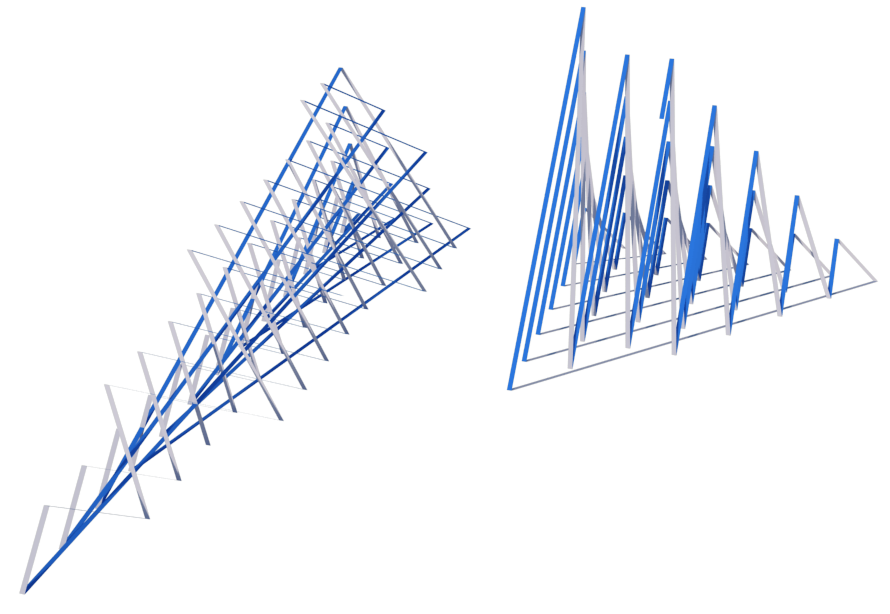
\includegraphics[width=0.8\textwidth]{enumerate2.png}
    \caption{Enumeration with repeated diagonalization (left), with hyperplanes (right) }%\bay{This figure is a little hard to interpret, but probably the most important visual feature is that one is narrower than the other.}}
  \label{enum3}
\end{figure}

The idea can be generally stated as grouping tuples by the distance to the origin with a norm. Then these tuples can be enumerated by arranging them monotonically increasing. Instead of planes one could imagine to use sphere surfaces. But it is probably much harder to calculate the n-th tuple in this case (and this is necessary as we will see later to make a proper Enum instance).

The enumeration with planes in the right picture of Figure \ref{enum3} generates tuples with a fair distribution of changes in the digits. It is especially fair in the beginning. An enumeration of n-tuples switches every digit once in the first n+1 values. For 3 tuples it is for example:
\begin{Verbatim}
[(0,0,0), (1,0,0), (0,1,0), (0,0,1), ...]
\end{Verbatim}
For higher values it becomes unfairer but other solutions (like hyperspheres) will maybe have much more complicated algorithms and formulas.
%\bay{Opportunity for more rigor! Or rigor mortis; your choice.}
While the 3d enumeration uses planes in higher dimensions hyperplanes have to be used. Thinking about this it becomes obvious that diagonals in 2d are hyperplanes as a hyperplane is a $(n-1)$-dimensional subset of a $n$-dimensional space that divides the space in two.

\section{Enum Instances}
%\bay{Signpost here. What are we doing now? What's the plan?}
The first experiments of this enumeration algorithm generated a list of tuples of Ints. Ideally we would like to replace Ints with arbitrary types as long as they can be enumerated. That of course also includes tuples itself. Haskell has a very nice feature called typeclass that permit the nesting of arbitrary tuples and values whose type have an \verb|Enum| instance. Take for example the \verb|Enum| instance for 2-tuples:

\begin{Verbatim}
instance (Enum a, Enum b, Eq a, Eq b, Bounded a, Bounded b)
                    => Enum (a, b) where
\end{Verbatim}
If \verb|a| is enumerable and \verb|b| is enumerable then the tuple \verb|(a,b)| is also enumerable. Because the values are enumerated from the low boundary to the high boundary and comparisons have to be made, \verb|a| and \verb|b| are also in \verb|Eq| and \verb|Bounded|. %\bay{Tangential, but an obvious thing to wonder is whether or not the Eq and Bounded constraints are strictly necessary.}\tkv{One has to make comparisons with minbound, so both classes are necessary, in my opinion obvious}
The goal is now to be able to write
\begin{Verbatim}
( enumFrom (0,(1,2),3) ) :: [(Word8,(Word8,Word8),Word8)]
\end{Verbatim}
This is an example for an arbitrary nesting, with arbitrary starting values, that evaluates to (you will see later why):
\begin{Verbatim}
[(0,(1,2),3), (0,(2,1),4), (0,(3,0),5), ...]
\end{Verbatim}


A type that should be enumerable can be made an instance of the \verb|Enum| typeclass by defining at least two functions:
\begin{Verbatim}
    toEnum           :: Int -> a
\end{Verbatim}
which returns a value of type \verb|a| to a number and
\begin{Verbatim}
    fromEnum         :: a -> Int
\end{Verbatim}
which returns a number to a value of type \verb|a|. There exist instances for primitive types like Char, Bool and Int.
The following functions are defined with \verb|toEnum| and \verb|fromEnum|, but can be overridden:

\begin{Verbatim}
    succ, pred       :: a -> a
    enumFrom         :: a -> [a]             -- [n..]
    enumFromThen     :: a -> a -> [a]        -- [n,n'..]
    enumFromTo       :: a -> a -> [a]        -- [n..m]
    enumFromThenTo   :: a -> a -> a -> [a]   -- [n,n'..m]
\end{Verbatim}

In our case we will overwrite \verb|succ| (the successor in the enumeration) and \verb|pred| (the predecessor), because they can be calculated more quickly than the default implementation:
\begin{Verbatim}
succ = toEnum . (`plusInt` oneInt)  . fromEnum
\end{Verbatim}

\section{succ, pred}
%\bay{The next sentence is unclear.}
In order to understand the following code take a look at the right picture  of Figure \ref{enum3}. Changes happen when a 0 is reached in the tuple. Because enumeration of arbitrary types should be possible, 0 is replaced by minBound. Instead of looking at a tuple it is faster to look only at the important digits: %\bay{I wonder if you can make this code look prettier by using guards or a match on equalities: \verb|match (a == minBound, b == minBound, c == minBound)|}\tkv{but for maximum speed one should check as few digits as possible. I think it can't be done prettier.}
\small
\begin{Verbatim}
succ (a,b,c) =
 if c == minBound then
  if b == minBound then
   if a == minBound then (succ a, b     , c     ) -- (0,0,0)
                    else (pred a, succ b, c     ) -- (a,0,0)
                   else  (a     , pred b, succ c) -- (a,b,0)
                 else
 if b == minBound then -- switching to the next hyperplane
 if a == minBound then (toEnum (fc+1), minBound, minBound) -- (0,0,c)
                  else (pred a  , toEnum (fc+1), minBound) -- (a,0,c)
                  else (a       , pred b       , succ c )  -- diagonals
  where
    fc = fromEnum c
\end{Verbatim}
The last tuple generates diagonals and every \verb|else| in the first half of this code generates a higher dimensional hyperplane.
The line \verb|(toEnum (fc+1), minBound, minBound)| makes a switch to a new hyperplane, that is one bigger in the sum of digits than the last hyperplane. Because the types in the tuple can be different from each other \verb|fromEnum c| and \verb|toEnum (fc+1)| have to be used instead of \verb|succ| and \verb|pred|. The function \verb|pred| for 3-tuples is implemented similarly:

\begin{Verbatim}
  pred (x,y,z) =
   if z == minBound then
    if y == minBound then
     if x == minBound then
       error "Enum.pred{(x,y,z)}: tried to take `pred' of minBound"
     else (minBound, minBound, toEnum (fx-1)) -- (fy,fz) was (0,0)
    else  (succ x  , minBound, toEnum (fy-1)) --     fz  was    0
   else   (x       , succ y  , pred z       )
    where
      fx = fromEnum x
      fy = fromEnum y
\end{Verbatim}
Here the line \verb|(minBound, minBound, toEnum (fx-1))| makes a switch to a lower hyperplane.

\subsection{Avoiding some typewriting}

%\bay{Not an editing comment per se, but if this journal was space constrained, this is the section I would cut.}\tkv{I hoped you could tell me if this is a good solution}

The function \verb|succ| could be defined for the other tuples in the same way, but this is a lot of typing for 15-tuples (the biggest tuple that is allowed). 
There is a pattern in the tuple that is produced when a certain pattern of zero or non-zero values in an inbound tuple occurs.
One can come up with functions that do the same as the upper \verb|succ| function when seeing an $n$-tuple as a list.
But a tuple can have all kinds of types and therefore is not compatible with an ordinary list. What to use? A heterogeneous list? One can also use a trick that transforms a tuple into a finite list-like structure and back:

\begin{Verbatim}
to5Tuple  ((((a,b),c),d),e)  = (a,b,c,d,e)
\end{Verbatim}

Then \verb|succ| can be defined like this:
\begin{Verbatim}
succ fz s ((x,y),z)
 | y /= minBound && z == minBound = ((x, pred y), succ z)
 | y == minBound && z == minBound = (succ fz False (x,y), z)
 | y /= minBound && z /= minBound = ((x,pred y), if s then succ z else toEnum (fz+1))
 | y == minBound && z /= minBound = (succ fz False (x,toEnum fz), minBound)
\end{Verbatim}
Here \verb|y| and \verb|z| should be imagined as single values while \verb|x| can be the list-like structure. 
Unfortunately the upper code gives a type error in Haskell (Occurs check: cannot construct the infinite type: t0 = (t0, a0)), which is understandable because the compiler can't know that this nesting terminates without a termination analyzer. In the expression \verb|((a,b),c)|  the value \verb|a| cannot stand for another tuple \eg \verb|(((d,e),b),c)| and the compiler does not know that we are not constructing an infinite type.
So we just define \verb|succ| for all tuples, like this:

\begin{Verbatim}[commandchars=\\\{\}]
\fbox{succ5} :: ( Enum a, Enum b, Enum c, Eq a, Eq b, Eq c,
           Bounded a, Bounded b, Bounded c) =>
         Int -> Bool -> ((\fbox{((a,b),c)},d),e) -> ((\fbox{((a,b),c)},d),e)
\fbox{succ5} fz s ((x,y),z)
| y /= minBound && z == minBound = ((x, pred y), succ z)
| y == minBound && z == minBound =  (\fbox{succ4} fz False (x,y), z)
| y /= minBound && z /= minBound =((x,pred y), if s then succ z else toEnum (fz+1))
| y == minBound && z /= minBound =  (\fbox{succ4} fz False (x,toEnum fz), minBound)
\end{Verbatim}
To define the other \verb|succ| functions one only has to change the number after the two \verb|succ|-functions in the body accordingly. 

I haven't found an easy way to do the same with \verb|pred|, because the last value in the tuple depends on values at various positions.
%This would become completely unusable if the cases for \verb|maxBound| (see next section) were introduced in there. %\ref{boundaries}).

\section {The size of enumeration hyperplanes}

The sizes of the enumeration hyperplanes are needed in order to assign numbers to tuples (\verb|toEnum|) or to find the place of a tuple in an enumeration  (\verb|fromEnum|).  From the right picture of Figure \ref{enum3} it can be seen that the 2D-hyperplanes consist of 1D-hyperplanes (diagonals).  Generally an $n$-dimensional space is enumerated with $(n-1)$-dimensional hyperplanes. These hyperplanes are again enumerated by $(n-2)$-dimensional hyperplanes, and so on. The size of an $n$-dimensional enumeration hyperplane can be deduced by looking at the two and three dimensional case.

The size of our 2D-hyperplane (a plane of diagonals) is a well known problem that Gauß solved at the age of nine:

\begin{equation}\label{gauss}
\begin{split}
& 1 +\\
&(1+1) +\\
&(1+1+1) + ... \\
& 1+2+3+4+5 ... + n  = \sum_{k=1}^{n} k =  n (n+1)/2
\end{split}
\end{equation}


A 3D-hyperplane consists of increasingly larger 2D-hyperplanes:

\begin{equation} \label{poly3d}
\begin{split}
& 1 +\\
&(1+2) +\\
&(1+2+3) + ... \\
& = \sum_{k=1}^{n}  k (k+1)/2 \\
& = \sum_{k=1}^{n} (\frac{k}{2} + \frac{k^2}{2}) = \frac{ n (n+1) }{2*2} + \frac{2n^3+3n^2+n}{6*2} 
\end{split}
\end{equation}

In (\ref{poly3d}), we sum over the polynomial of the Gauß sum (\ref{gauss}).

To calculate the sum of $k^2$'s, the Bernoulli formula for sums of powers was used:

\begin{equation} \label{bernoulli}
\boxed{
\sum_{k=1}^{n-1} k^p = \frac{1}{p+1} \sum_{j=0}^{p} \binom{p+1}{j} \beta_{j} n^{p+1-j}
}
\end{equation}

Applying this pattern again leads to the size of a 4D-hyperplane:

\begin{equation}\label{poly4d}
\begin{split}
 & 1 +\\
 &(1+(1+2) )+ \\
 &(1+(1+2)+(1+2+3)) + ... = \sum_{k=1}^{n} (\frac{ k (k+1) }{2*2}  + \frac{2k^3+3k^2+k}{6*2})
\end{split}
\end{equation}

\subsection {Calculating it}

The last section showed that the size of a hyperplane can be given with a polynomial. The common way to represent a polynomial is to only use its coefficients. Therefore a function is needed to evaluate a polynomial in $n$:
\small
\begin{Verbatim}
       polynomial :: Int -> [Rational] -> Rational
       polynomial n coeffs = foldr (+) 0 (zipWith nPowerP coeffs [1..])
         where nPowerP a_j p = a_j * (fromIntegral (n^p))
\end{Verbatim}

The coefficients of a polynomial in $n$ that results from $\sum_{k=1}^{n-1} k^p$ are needed. At position $n^{p+1-j}$ this is:

\begin{equation} \label{coefficient}
\mbox{coefficient}(j) = \frac{1}{p+1} \binom{p+1}{j} \beta_{j}.
\end{equation}

The \verb|combinat| library, which can be found on Hackage, provides some parts of the Bernoulli formula: the Bernoulli numbers $\beta_{j}$ and the binomial coefficient. With this, a part of the Bernoulli formula can be implemented by:

\small
\begin{Verbatim}
sumOfPowers :: Int -> [Rational]
sumOfPowers p = reverse [ (bin j) * (ber j) / ((fromIntegral p)+1) | j <- [0..p] ]
  where bin j = fromIntegral (binomial (p+1) j)
        ber j | j == 1 = negate (bernoulli j) -- see wikipedia entry
              | otherwise = bernoulli j
\end{Verbatim}

Because of the $-j$ in $n^{p+1-j}$, a \verb|reverse| is needed.
We apply this formula to a polynomial with increasing degree: first $k$, then $\frac{k}{2} + \frac{k^2}{2}$, ....

The size of an n-dimensional hyperplane can be calculated by repeatedly applying the Bernoulli formula (\verb|map sumOfPowers|) to the $n^p$ after the coefficients of a polynomial and adding the coefficients (\verb|merge|):

\small
\begin{Verbatim}
hyperplaneSize :: Int -> Int -> Int
hyperplaneSize dim n = round (genPolynom 1 [1])
  where genPolynom :: Int -> [Rational] -> Rational
        genPolynom d coeffs | d == dim  = polynomial n coeffs
                            | otherwise = genPolynom (d+1)
                              (merge coeffs (map sumOfPowers [1..(length coeffs)]))

merge coeffs ls = foldr myZip [] multiplied_ls
  where multiplied_ls = zipWith (\c l -> map (c*) l) coeffs ls
        myZip (l0:l0s) (l1:l1s) = (l0+l1) : (myZip l0s l1s)
        myZip a b = a ++ b
\end{Verbatim}

\subsection{fromEnum}

The function \verb|fromEnum| takes a tuple and gives back an integer. If we want to calculate \eg \ \verb|fromEnum (True,'a',2)| we first apply \verb|fromEnum| to every argument: 

\begin{Verbatim}
fromEnum (fromEnum True, fromEnum 'a', fromEnum 2)
\end{Verbatim}

The tuple now only consists of integers (here \verb| fromEnum (1,97,2)|).
Using \verb|fromEnum| at every digit of the tuple, a general function \verb|fe| can be constructed that transforms an arbitrary sized list of integers: %\bay{But what is \verb|fe| actually doing?}

\begin{Verbatim}
  fromEnum (a,b,c) = fe [fromEnum a, fromEnum b, fromEnum c]
\end{Verbatim}

To understand how \verb|fe| works recall that a hyperplane consists of all tuples whose sum of digits is constant. For the upper 3-tuple there is one 2d-plane that is located at the sum of the three integers. All the hyperplanes below this one have to be summed up. To calculate a tuple's position inside the 1d-hyperplane (diagonal) of this plane, the plane is projected to a lower dimension by setting one coordinate to zero. Instead of planes in 3d we now have diagonals in 2d. The sum of the tuple values of this smaller tuple give us again a hyperplane and the  hyperplane-sizes below have to be added to the overall sum. This process ends with a position inside of a 1d-line.

The decision which dimension to set to zero is a degree of freedom but it has to be used consistently with \verb|toEnum|, \verb|succ| and \verb|pred| obviously. There are two ways to do this in 2D, three ways in 3D, generally $n$ ways in an $n$-dimensional space. %\bay{I don't think this is strictly true; setting one coordinate to zero corresponds to projecting onto that plane; but there are infinitely many planes and thus infinitely many projections.  In the discrete case, many of these may not be interesting, but it is a thought.}

In the last section we saw how to calculate the size of the $n$th enumeration hyperplane of a $d$-dimensional space. The function \verb|fe| uses lists of these sizes and an increasingly larger sum of hyperplanes:

\begin{Verbatim}
ssizes d = [ sum (take n sizes) | n <- [1..] ]
  where sizes = [ hyperplaneSize d i | i <- [0..] ]

summedSizes :: Int -> Int -> Int
summedSizes dim n = (ssizes dim) !! n
\end{Verbatim}

For the upper 3-tuple, we always set the first value to zero, and thus calculate:

\begin{Verbatim}
  (summedSizes 2       (a1+b1+c1) ) +     -- a1 = fromEnum a
  (summedSizes 1          (b1+c1) ) +     -- b1 = fromEnum b
                              c1          -- c1 = fromEnum c
\end{Verbatim}

For all dimensions:
\begin{Verbatim}
fe [x] = x
fe (x:xs) = ( summedSizes (length xs) (foldr (+) 0 (x:xs)) ) + (fe xs)
\end{Verbatim}

\subsection {toEnum }
To calculate \verb|toEnum|, we have to invert the upper process. If \verb|toEnum| gets the argument \verb|n|, and the tuple has dimension $d$, then we search for where $n$ is located between the sums of hyperplanes by summarizing the  smaller hyperplanes until \verb|n| is reached and continue with the lower dimensions. But instead of values for each tuple position we get sums of subtuple values. To see how to extract values at each position from the sums, look again at the example of a 3-tuple: To get \verb|a1|, it is enough to know the two sums \verb|(a1+b1+c1)| and \verb|(b1+c1)| and calculate the difference:

\begin{Verbatim}
differences :: [Int] -> [Int]
differences [x] = [x]
differences (x:y:ys) = (x-y) : (differences (y:ys))
\end{Verbatim}

But first we calculate each of these sums (like the one belonging to \verb|a1+b1+c1|), put them in the list \verb|planes| and also remember the \verb|rest| for the next round:

\begin{Verbatim}
hplanes :: Int -> ([Int],Int) -> ([Int],Int)
hplanes d (planes,rest) = ((fst hp):planes, snd hp)
  where hp = hyperplane d rest
\end{Verbatim}

\begin{Verbatim}
hyperplane dim n = ( (length s) - 1, n - (if null s then 0 else last s) )
  where s = filterAndStop [ summedSizes (dim-1) i | i <- [0..] ]
        filterAndStop (x:xs) | x <= n     = x : (filterAndStop xs)
                             | otherwise = []
\end{Verbatim}

\verb|te| uses the upper functions and works for an arbitrary dimensioned tuple:

\begin{Verbatim}
te :: Int -> Int -> [Int]
te dim n = differences $ reverse $ fst $ foldr hplanes ([],n) [1..dim]
\end{Verbatim}


\section{Reaching boundaries}
Until now only tuples with large sets were enumerated where it takes a long time to reach boundaries. But if tuples with Bools are enumerated (or with only four elements like in figure \ref{enum2bounded}), boundaries are quickly reached. Notice that in figure \ref{enum2bounded} the diagonals are enumerated from bottom right to top left and only half of the last line is subtracted. For non-quadratic rectangles it is also easier to subtract triangular shapes than to calulate the red area (especially in higher dimensions as we see later).

\begin{figure}[htbp]
  \centering
    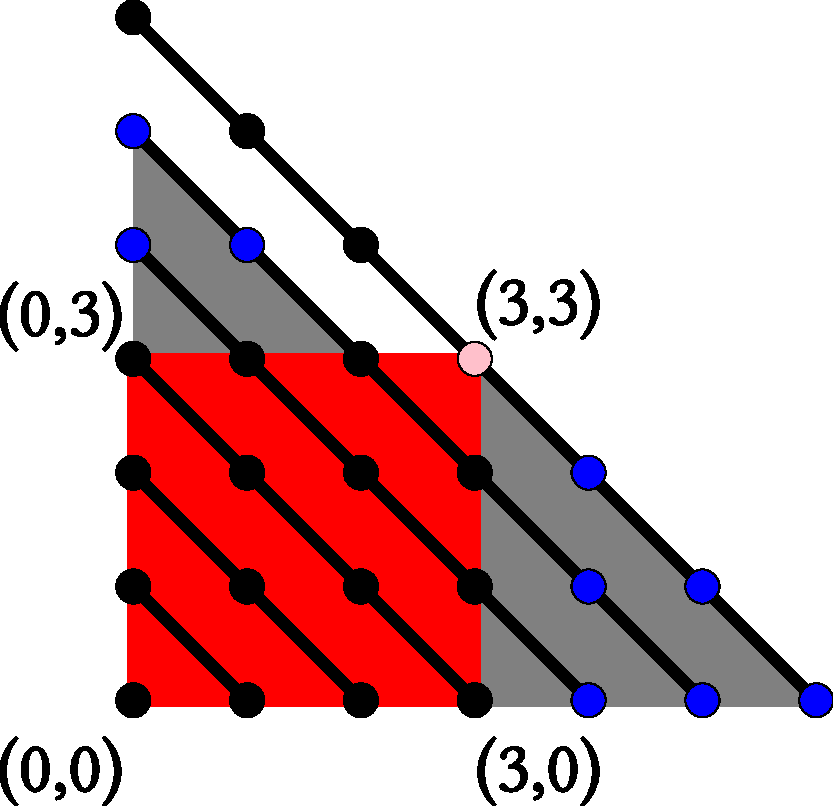
\includegraphics[width=0.3\textwidth]{en.pdf}
    \caption{Reaching boundaries in two dimensions }
  \label{enum2bounded}
\end{figure}

Figure \ref{enum3bounded} shows boundaries in 3d where the enumeration planes in 3d form a tetrahedron starting at the origin. From this base tetrahedron three tetrahedra have to be subtracted that are translated by the size of the boundary in the respective dimension (also try to imagine a book shape instead of a cube in the picture). The intersections of these three tetrahedra make it necessary to add again three smaller tetrahedra that start at two added boundaries. In the former sections we could see a pattern from the 2d to the 3d case and deduce a general pattern. There seems to be no obvious pattern in this case, as we don't know how hypertetrahedra intersect in higher dimensions.

\begin{figure}[htbp]
  \centering
    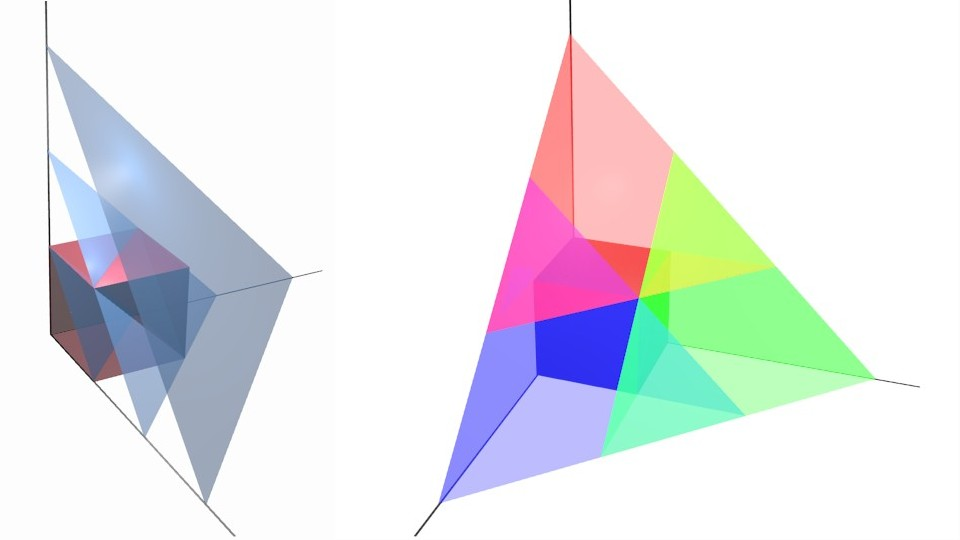
\includegraphics[width=0.9\textwidth]{planes.jpg}
    \caption{Left: Enumeration planes that intersect a bounded space. Right: The tetrahedra that have to be subtracted (red, green, blue) and added again (violet, yellow, blue-green) }
  \label{enum3bounded}
\end{figure}

\subsection{Intersections of hypetretrahedra}
To get an idea of how many intersections there are we generate a 5d-hypertretrahedron (\verb|all5s| is an enumeration from (0,0,0,0,0)):

\begin{Verbatim}
set5 s = [ (a,b,c,d,e) | (a,b,c,d,e) <- (take 5000 
           (all5s :: [(Word8,Word8,Word8,Word8,Word8)]) ),  a+b+c+d+e <= s ]
set510 = set5 10
\end{Verbatim}

Then we translate this hypertetrahedron by the same length in each dimensions respectively and look at all combinations of intersections.
The library Hasklell-for-maths gives us a function that generates all subsets of size k:

\begin{Verbatim}
combinationsOf 0 _ = [[]]
combinationsOf _ [] = []
combinationsOf k (x:xs) =
  map (x:) (combinationsOf (k-1) xs) ++ combinationsOf k xs
\end{Verbatim}

The following function returns sets of indices to hypertretrahedra where the index specifies in which dimension they were translated.

\begin{Verbatim}
intersectionSets = concat $ map (\k -> combinationsOf k [0..4] ) [2..5]
\end{Verbatim}

has the value

\begin{Verbatim}
[[0,1],[0,2],[0,3],[0,4],[1,2],[1,3],[1,4],[2,3],[2,4],[3,4],
[0,1,2],[0,1,3],[0,1,4],[0,2,3],[0,2,4],[0,3,4],[1,2,3],[1,2,4],
[1,3,4],[2,3,4],[0,1,2,3],[0,1,2,4],[0,1,3,4],[0,2,3,4],
[1,2,3,4],[0,1,2,3,4]].
\end{Verbatim}

If we do an \verb|intersectionTest| with
\begin{Verbatim}
intersectionTest =
  filter (\set -> (length (intersection set)) > 1) intersectionSets
intersection set = intersectAll (map translated set)
intersectAll set = foldr intersect (head set) (tail set)
translated dim = map (add5 (tr5 dim 5)) set510
  where add5 (a,b,c,d,e) (f,g,h,i,j) = (a+f,b+g,c+h,d+i,e+j)
\end{Verbatim}
we get $\binom{5}{2} = 10$ intersections:

\begin{Verbatim}
[[0,1],[0,2],[0,3],[0,4],[1,2],[1,3],[1,4],[2,3],[2,4],[3,4]]
\end{Verbatim}

In higher dimensions it seems that all intersections of 2 hypertretrahedra exist but three or more hypertetrahedra are not intersecting in more than one point.

\subsection{fromEnum with boundaries}
In the bounded case \verb|fromEnum| is calculated nearly in the same way as in the previous sections. Looking again at figure \ref{enum3bounded} there is a top hyperplane below which the other hyperplanes are summed up. They form the base hypertetrahedron from which \verb|d| tetrahedra (as many as the tuple has dimensions) have to be subtracted (\verb|sum (map intersection xs)|) and because they also intersect between each other hypertetrahedra have to be added again (\verb|(sum intersection2)|):

\begin{Verbatim}
fe [(x,b)] = x
fe xs start = ( (summedSizes (length xs) s)
               - (sum (map intersection xs))
               + (sum intersection2) )
        + (fe (tail xs) false)
  where s = foldr (+) 0 (x:xs)
        intersection (x,b) = if s > b then summedSizes (length xs) (s-b)
                                      else 0
        intersection2 = map (\[x,y] -> inter (xs!!x) (xs!!y) )
                            (combinationsOf 2 [0..((length xs)-1)]))
        inter (_,b0) (_,b1) = if s > b0 + b1
                                then summedSizes (length xs) (s-b0-b1)
                                else 0
\end{Verbatim}

In the upper code we have to introduce the bool argument \verb|start| to cope with a strange effect. Although our experiment showed that there are only intersections of at most 2 hypertetrahedra, this is only true in the beginning. Once we project the tuple to one dimension below, there are more intersections.
Consider this example: In 4 dimensions we have to subtract 4 hypertetrahedra. These hypetretrahedra are the original 4d enumeration, translated in each of the 4 dimensions respectively. \eg
\begin{Verbatim}
(1,0,0,0)
(0,1,0,0)
(0,0,1,0)
(0,0,0,1)
\end{Verbatim}

This 4d enumeration consists of repeated 3d enumerations. If we are only interested in the last 3d object in 4d space (the hyperplane that belongs to the sum of all digits), we get four 3d objects in 4d space. How do they look like? We can project them on dimension lower by setting one dimension to zero. Three 3d objects are still translated, but one is set to the origin. So the 3d objects are in every of the 4 corners of a normal 3d-tretrahedron. That is one tetrahedron more than in right part of figure \ref{enum3bounded}. But does this mean that if we start with a 10 dimensional tuple, the plane in 2d has a very complicated shape? Fortunately with every dimension we go lower the hypertetrahedron that is at the origin is parallel to the enumeration and therefore does not influence the intersections at the top hyperplane where we go next. But instead of only at most 2 hypertetrahedra intersecting, all hyperplanes intersect. Try to imagine this with 4 hypertetrahedra in 4 corners and arbitrary sizes.

%In the upper code you can see that the size of the boundaries and the hyperplane of the tuple are enough to calculate these intersections. Unfortunately the upper formula can not be used recusively and the function \verb|feSub| has to be introduced. The dimension below the one \verb|fe| has been called with can have intersections with more than two hypertretrahedra.


\subsection{toEnum with boundaries}

\subsection{succ,pred}

%\bay{We're done? Say so!}

\section{Previous work and Conclusion}

\cite{auth:tuple-gen}
\cite{rationals}
\cite{knuth}

\bay{Maybe expand this paragraph a little bit, and make it more cohesive.}
The idea to enumerate tuples this way is about year old. \bay{It may be safer to hedge bets by saying that you weren't aware of any prior work.} While writing \verb|Enum|-Instances it seemed interesting enough to write an article about it. So far I could not find a reference mentioning it (\eg\ Donald Knuth: Generating All Tuples and Permutations). I think it can save some time in combinatorial problems or when one has to chose an option among several possibilities, \eg\ in generating a user interface.

\subsection{Appendix}

The images were generated with \verb|collada-output| and \verb|diagrams|.

\begin{verbatim}
main = B.writeFile "test.svg" $ toLazyByteString $
                renderDia SVG (SVGOptions (Dims 100 100)) (enum2 ||| enum3)

-- 2D enumeration

enum2 =  ((stroke ( mconcat $ translatedPoints)) 
             # fc black # fillRule EvenOdd )
      <> enumLines
      <> ( translate (-1,-1) $ text' "(0,0)")
      <> ( translate (4 ,-1) $ text' "(4,0)")
      <> ( translate (-1, 4.25) $ text' "(0,4)")

translatedPoints = map (\v -> translate v (circle 0.15) ) points

points = map (\(x,y) -> (fromIntegral x, fromIntegral y))
                              $ take 15 ( all2s :: [(Word8,Word8)] )

enumLines = mconcat $ 
            colorize (map enumLine (pointList points []) # lw 0.1)
 where enumLine l = fromVertices (map P l)
       pointList []         l = [l]
       pointList ((0,y):ps) l = ((0,y):l) : ( pointList ps [] )
       pointList ((x,y):ps) l = pointList ps (l ++ [(x,y)])

colorize = zipWith (\c d -> d # lc c) [yellow,red,green,blue,orange]

text' t = stroke (textSVG t 0.8) # fc black # fillRule EvenOdd
\end{verbatim}

\bibliography{tuples}

\end{document}
